\chapter{Evaluation} % Main chapter title

\label{Chapter6} % For referencing the chapter elsewhere, use \ref{Chapter1} 

\lhead{Chapter 5. \emph{Evaluation}}
This chapter presents evaluation of the approach presented in Chapter \ref{Chapter3} to answer the proposed research questions. 

\section{Evaluation setup}
\label{evalsetup}
This research evaluates 5 open source web applications as described in Table \ref{appcandidates}. Selecting suitable candidates which satisfy the project requirement has been a challenge, since not many organizations have open source Selenium test repositories. 


% \begin{tabulary}{\textwidth}{|c|c|c|c|c|c|}
% \hline
% Application&  Language&  Page-objects&  \#Test classes&  \#Test methods&  LOC\footnote{Without comments and blank lines using the tool CLOC (\url{cloc.sourceforge.net})}  \\
% \hline
%  Jenkins\footnote{\url{https://github.com/jenkinsci/acceptance-test-harness}}&  Java&56&  &  &    \\
% \hline
% Moodle\footnote{\url{https://github.com/moodlehq/functional-test-suite}}&  Java&  13&  &  &    \\
% \hline
% Mozilla Addons\footnote{\url{https://github.com/mozilla/Addon-Tests/}} &  Python&  17&  &  &    \\
% \hline
% Mozilla Marketplace\footnote{\url{https://github.com/mozilla/marketplace-tests}} &  Python&  12&  3&  &  \\
% \hline
% Mozilla.org\footnote{\url{https://github.com/mozilla/mcom-tests}} &  Python&  16&  16&  &   \\
% \hline
% \caption{Application Candidates}
% \label{app-candidates}
% \end{tabulary}
\resizebox{10cm}{!}{
\begin{tabular}{l*{6}{l}r}
\\
\hline
Application              & Language & \#Page-objects & \#Tests & \#LOC\footnote{Without comments and blank lines using the tool CLOC (\url{cloc.sourceforge.net})} & F  \\
\hline
Jenkins & Java & 4 & 0 & 2 & 10  \\
Moodle            & Java & 3 & 0 & 3 &  8 \\
Mozilla Addons           & Python & 2 & 1 & 3 &  7  \\
Mozilla Marketplace     & Python & 2 & 1 & 3 &  5   \\
Mozilla.org     & Python & 2 & 1 & 3 &  5   \\
\hline
% \caption{Application Candidates}
\label{app-candidates}
\end{tabular}}
\begin{flushleft}
\resizebox{14cm}{!}{
\begin{tabular}{l*{6}{l}r}
\\
\hline
Application              & Domain & \#Major Versions & \#Minor Versions \\
\hline
Jenkins & Continuous Integration tool & 4 & 0   \\
Moodle            & Course Management System & 1 & 12  \\
Addons           & Software Add-ons vendor & 3 & 1  \\
Marketplace     & Software Apps vendor  & 4 & 1   \\
Mozilla.org     & Mozilla Project Homepage & 2 & 1   \\
\hline
% \caption{Application Candidates}
\label{appcandidates}
\end{tabular}}
\end{flushleft}
% \end{table}
% \end{tiny}
% \end{savenotes}


\begin{figure}[ht!]
\centering     %%% not \center
\vspace{-2mm}\subfigure[AUT version $V_{1}$]{\label{rob:amo}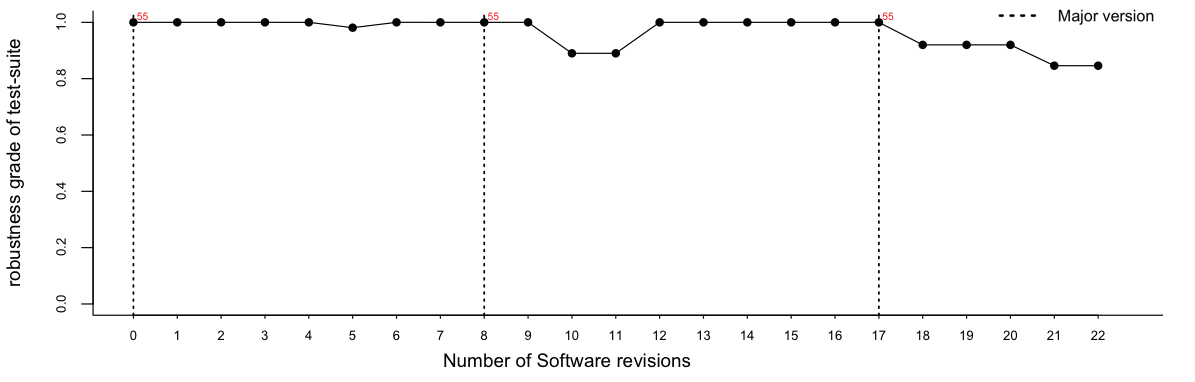
\includegraphics[width=\linewidth,height=3.3cm]{./Figures/amo-rq1}}
\vspace{-2mm}\subfigure[AUT version $V_{1}$]{\label{rob:fireplace}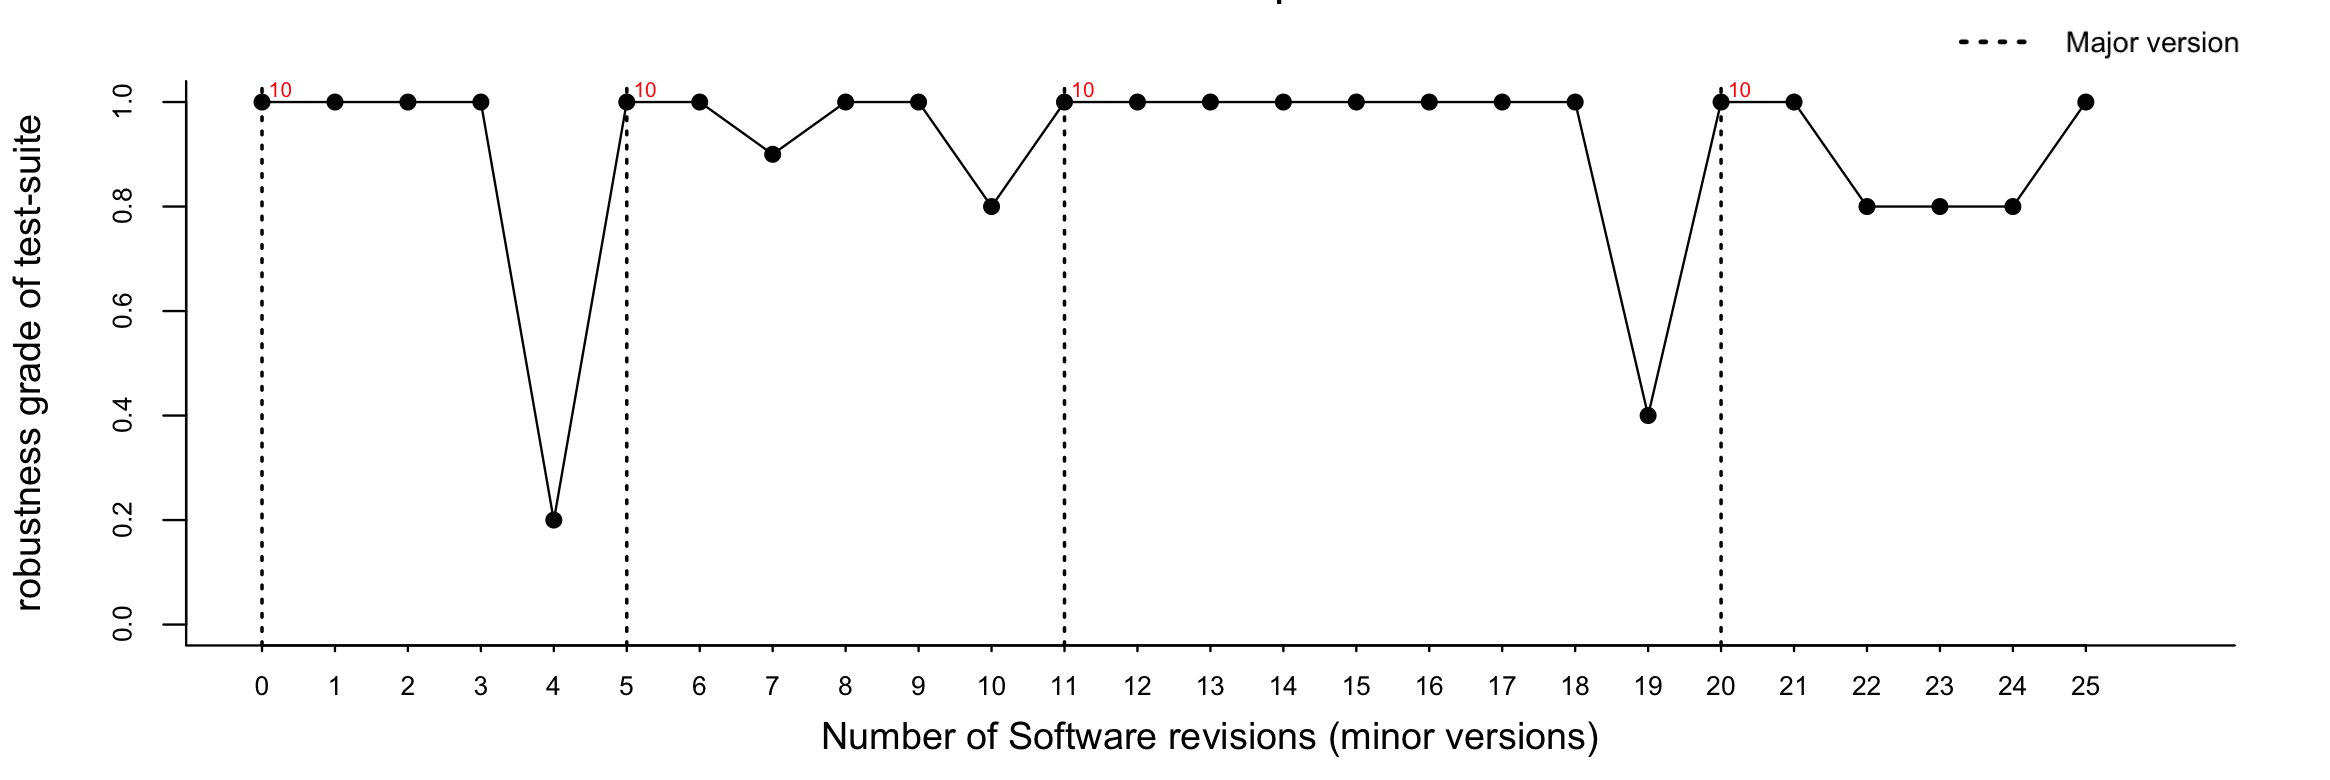
\includegraphics[width=\linewidth,height=3.3cm]{./Figures/fireplace-rq1}}
\subfigure[AUT version $V_{0}$]{\label{rob:moodle}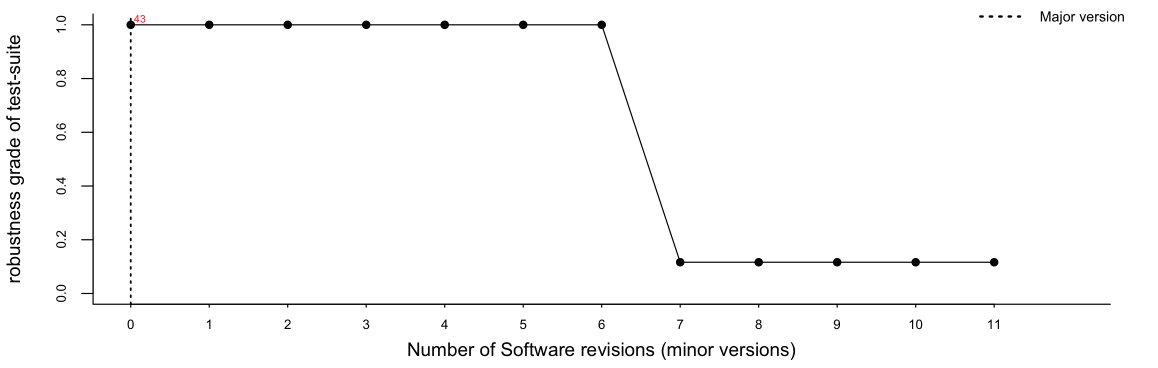
\includegraphics[width=\linewidth,height=3.3cm]{./Figures/moodle-rq1}}
\vspace{-2mm}\subfigure[AUT version $V_{1}$]{\label{rob:amo}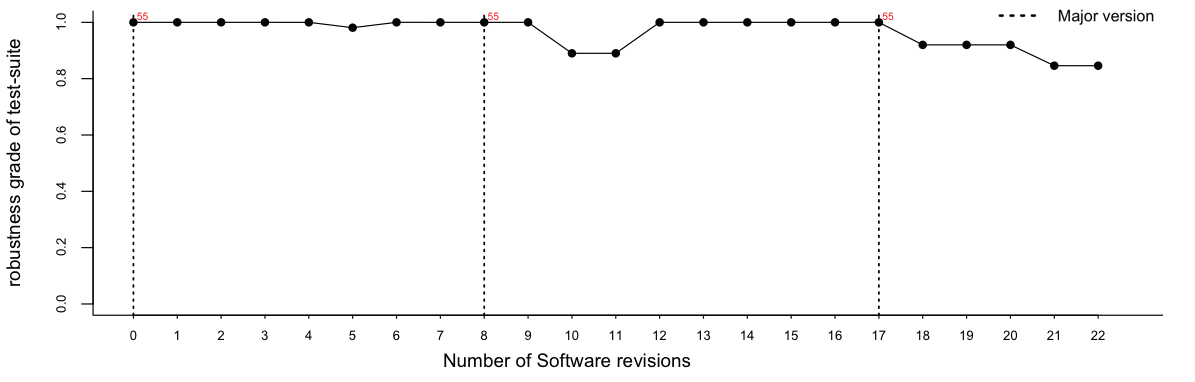
\includegraphics[width=\linewidth,height=3.3cm]{./Figures/amo-rq1}}
\vspace{-2mm}\subfigure[AUT version $V_{1}$]{\label{rob:fireplace}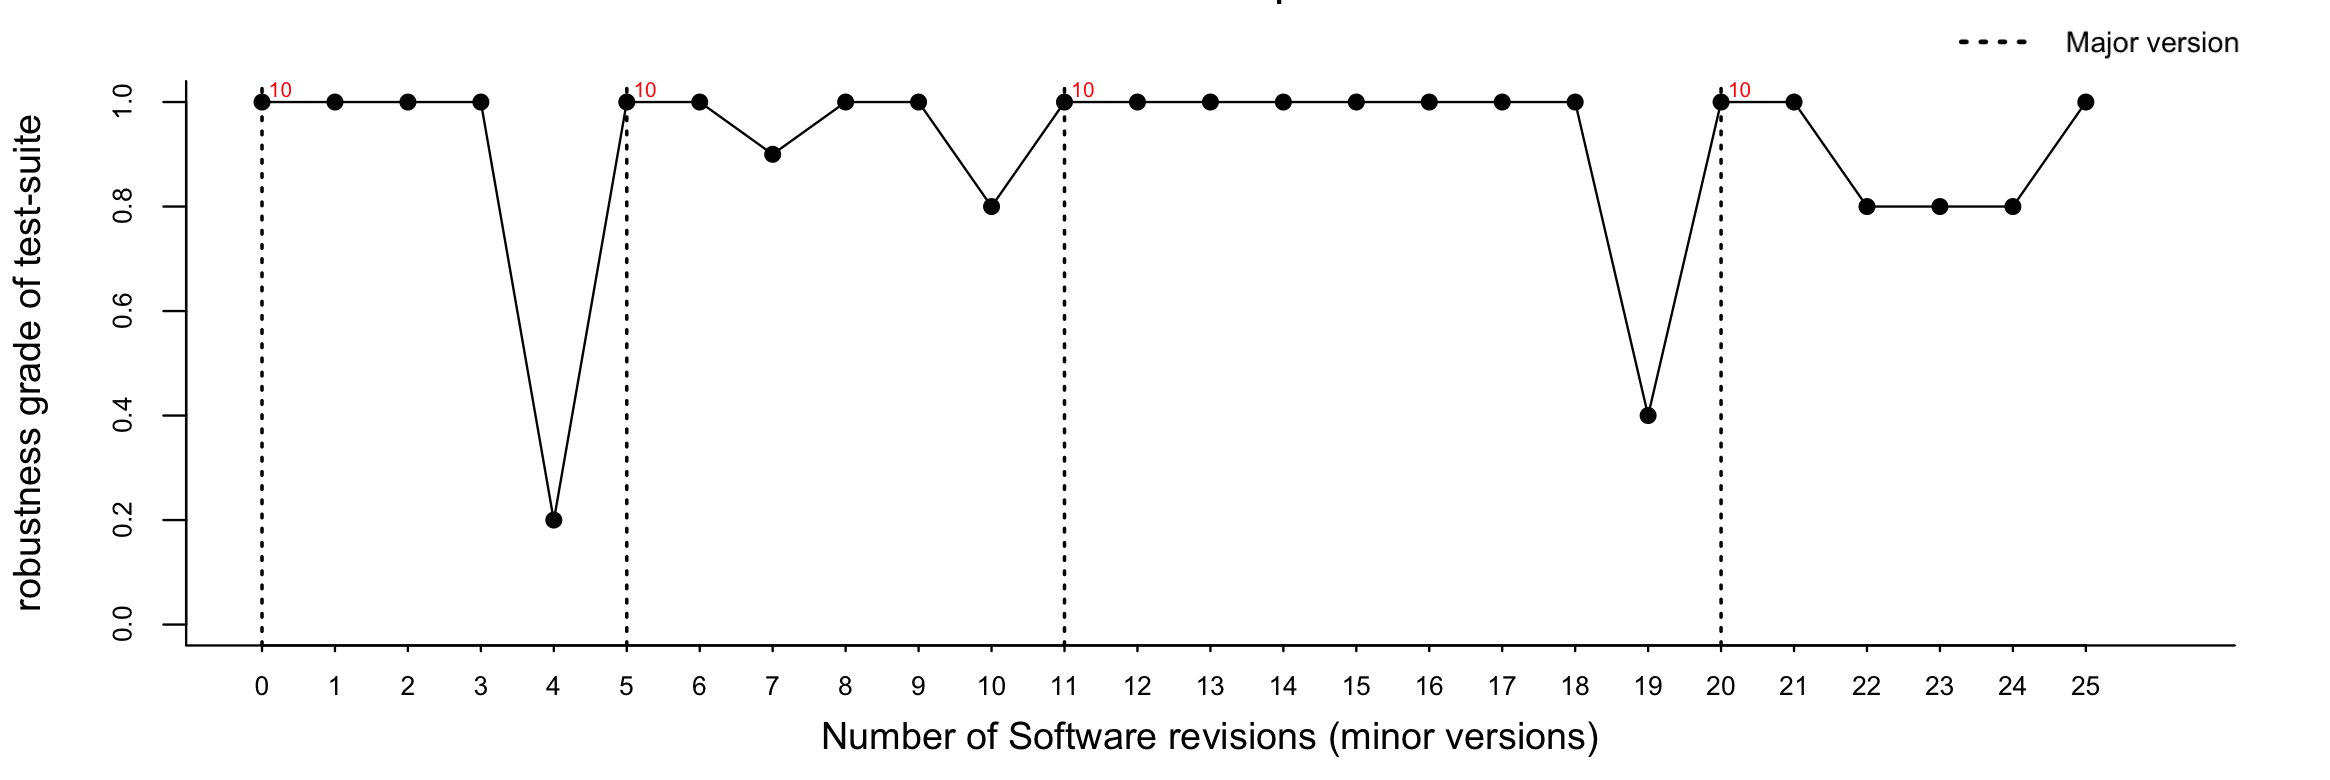
\includegraphics[width=\linewidth,height=3.3cm]{./Figures/fireplace-rq1}}
\captionsetup{justification=justified,
singlelinecheck=false}
\caption{Robustness grade Robustness grade Robustness grade Robustness grade Robustness grade Robustness grade Robustness grade Robustness grade Robustness grade Robustness grade Robustness grade Robustness grade }
\label{fig:robustnessplots}
\end{figure} 